I wrote the DAG generator that we used thanks to the OCamlgraph Librairy. The Dag Generator is a functor with signature :
\begin{lstlisting}
module type Elem = 
sig
  type t
  (** [init n] initializes the Random element generator where [n] is a seed
  *)
  val init : int -> unit
  (** [next_item n] gives back a new element where [n] is the size of the new element
  *)
  val next_item : int -> t
end
module Make :
  functor (B : Graph.Sig.I) ->
    functor (L : Elem with type t = B.V.t) ->
      sig
	(** [alea n h t seed p] is the function that produces a dag
	and the biggest element of this dag where [n] is the
	number of nodes of the dag and [h] is the high of the dag
	and [t] is the size of the element in the dag and [seed]
	is the seed used to initialize the element generator and
	[p] is the probability that a node of high i is the son of
	a node of high (i-1)
	*)
	val alea : int -> int -> int -> int -> float -> B.t * B.V.t
      end
\end{lstlisting}

\begin{figure}[H]
 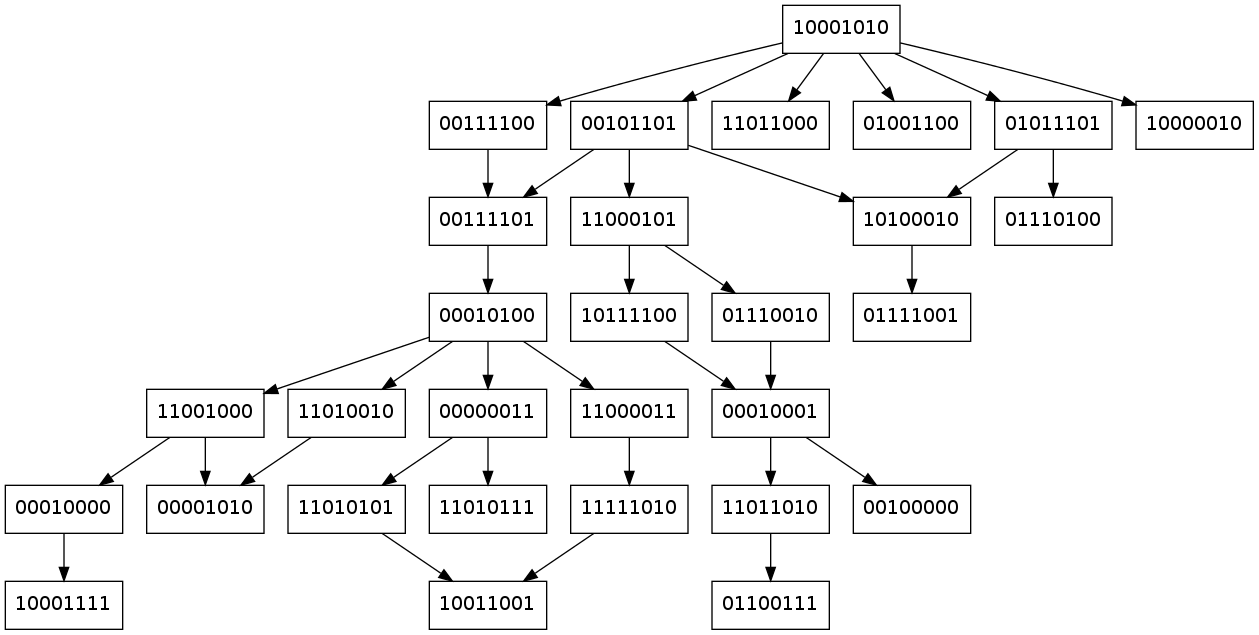
\includegraphics[width = \textwidth]{./image/DagGen/output025.png}
 \caption{DAG generated with $p=0.25$} \label{DAGgen}
\end{figure}
\begin{figure}[H]
 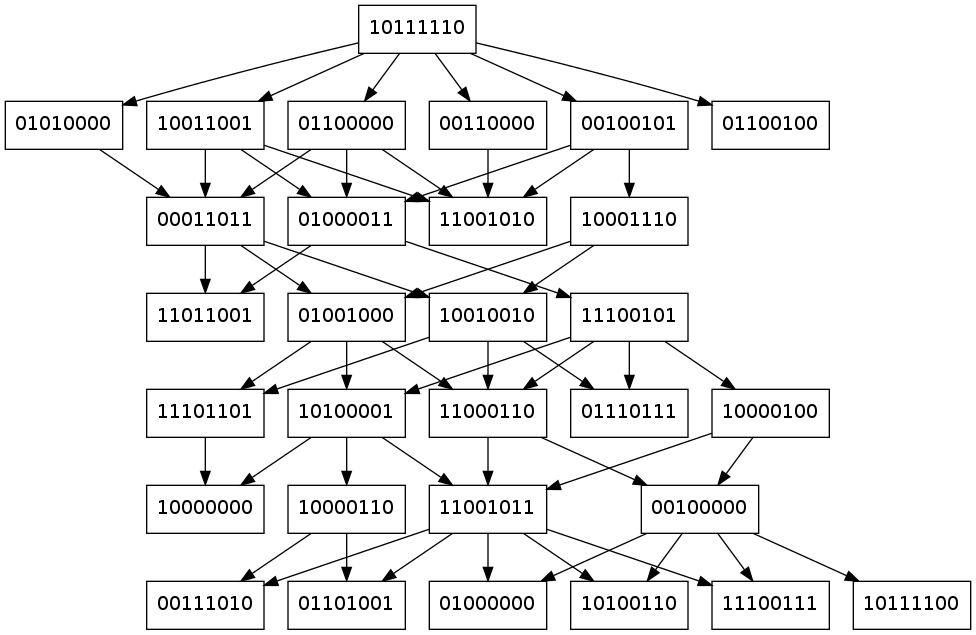
\includegraphics[width = \textwidth]{./image/DagGen/output05.png}
 \caption{DAG generated with $p=0.5$}
\end{figure}
\begin{figure}[H]
 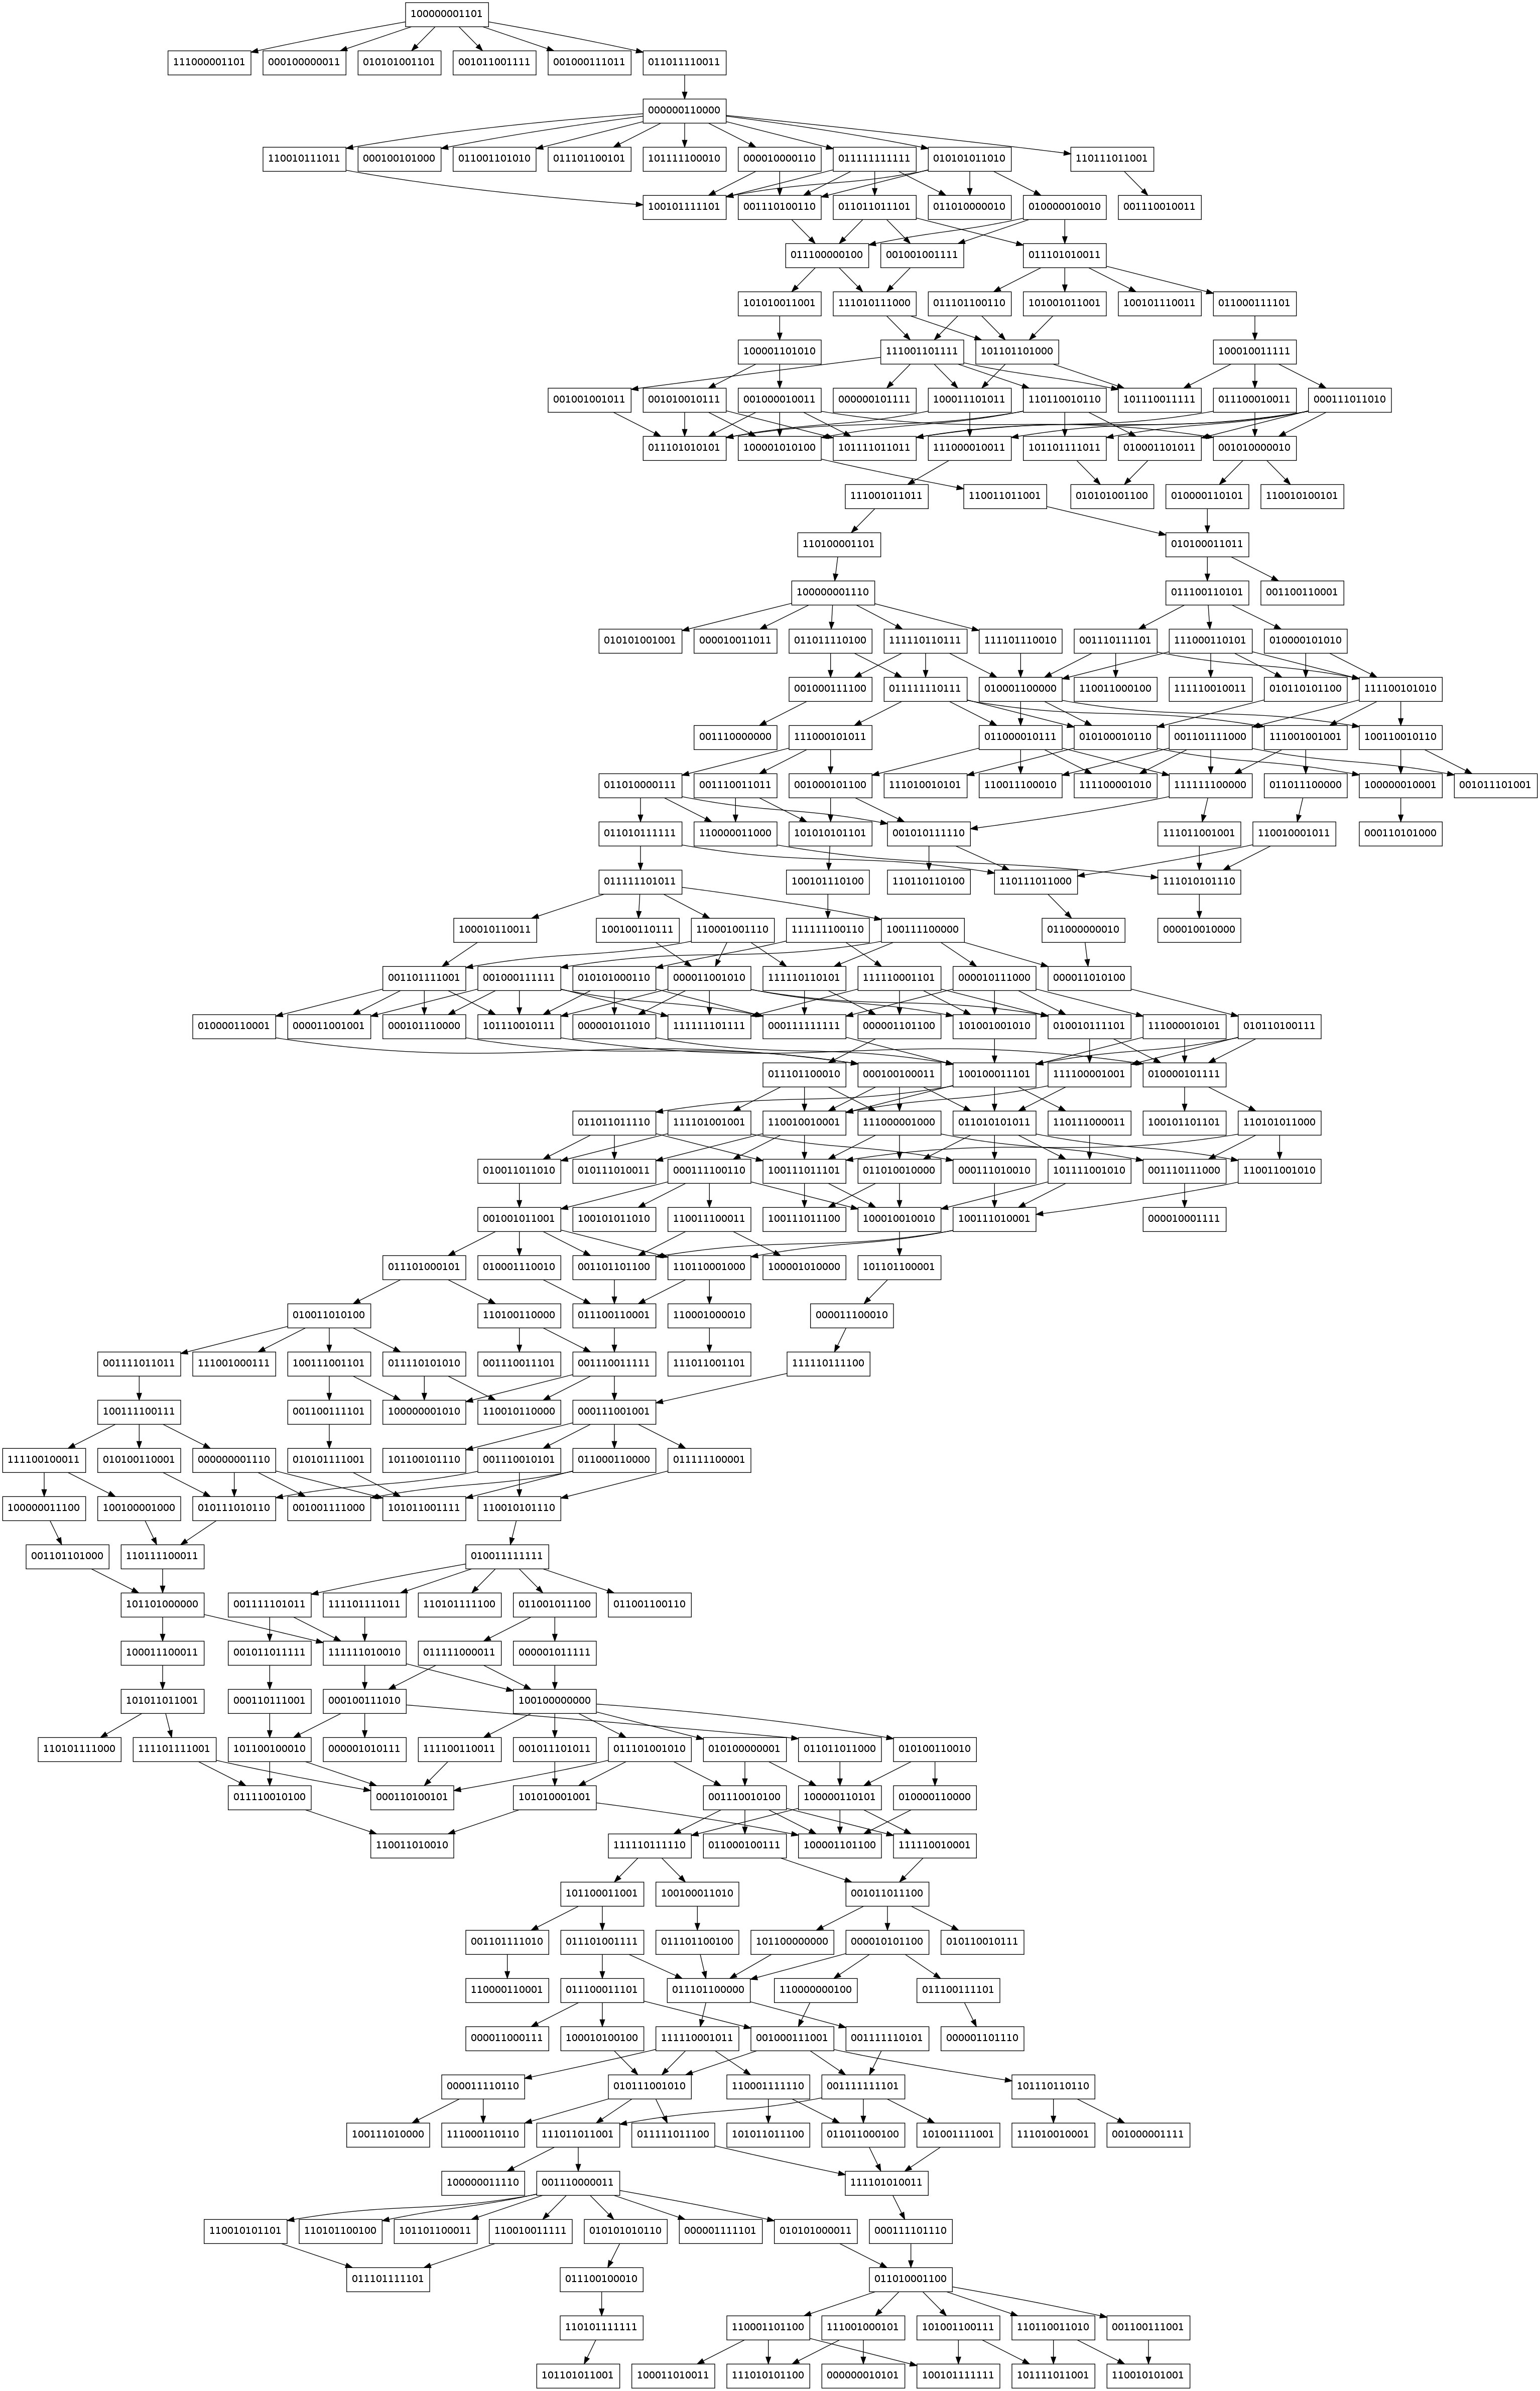
\includegraphics[width = \textwidth]{./image/DagGen/outputbig.png}
 \caption{A full git tree}
\end{figure}